\section{Глава для тестирования ссылок на объекты приложений из основного текста}
\sectionmark{Глава для тестирования ссылок на объекты приложений из основного текста}

\subsection{Ссылки на таблицы}

Таблица~\ref{t_main:1} простая.

\begin{longtable}{|p{60mm}|p{100mm}|}
  \caption{Простая} \label{t_main:1} \\
  \hline
  \multicolumn{1}{|p{60mm}|}{\centering Обозначение} &
  \multicolumn{1}{p{100mm}|}{\centering Наименование} \\\hline
  \endfirsthead
  \caption*{Продолжение таблицы \ref{t_main:1}} \\
 \hline
  \multicolumn{1}{|p{60mm}|}{\centering Обозначение} &
  \multicolumn{1}{p{100mm}|}{\centering Наименование} \\\hline
  \endhead
   1    &   2   \\ \hline
   3    &   4   \\ \hline
   5    &   6   \\ \hline
\end{longtable}

Таблица~\ref{appendix:t:1} такая же как таблица~\ref{t_main:1}.




\subsection{Ссылки на рисунки}

На рисунке~\ref{p:func_in2_1_main} приведено то же, что и на рисунке~\ref{p:func_in2_1}

\begin{figure}[!h]
  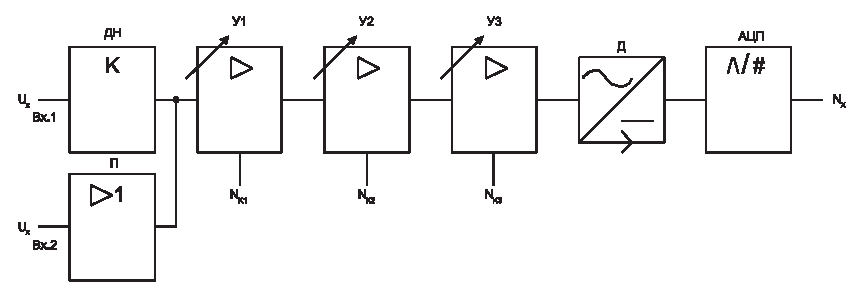
\includegraphics[width=1\textwidth]{./about/func_in}
  \caption{Функциональная схема измерителя напряжения ИН2, необходимая для демонстрации возможностей включения рисунков и корректного переноса подрисуночной подписи}
  \label{p:func_in2_1_main}
\end{figure}



\subsection{Ссылки на формулы}


Уравнение~(\ref{eq:n_x_main}) такое же как~\eqref{eq:n_x}:
\begin{eqnarray}
N'_x=U_xK_1(1+\delta_1)K_{\text{У1}}(1+\delta_{\text{У1}})K_{\text{У2}}(1+\delta_{\text{У2}})
\eqnewline{\times}
	K_{\text{У3}}(1+\delta_{\text{У3}})K_{\text{Д}}(1+\delta_Д)K_{\text{АЦП}}(1+\delta_{\text{АЦП}}),
\label{eq:n_x_main}
\end{eqnarray}
\par где $\delta_1$~– погрешность коэффициента передачи предварительного блока (делителя или повторителя);
\par $\delta_{\text{У1}}$~– погрешность коэффициента передачи усилителя У1;
\par $\delta_{\text{У2}}$~– погрешность коэффициента передачи усилителя У2;
\par $\delta_{\text{У3}}$~– погрешность коэффициента передачи усилителя У3;
\par $\delta_{\text{АЦП}}$~– погрешность коэффициента передачи АЦП;
\par $\delta_\text{Д}$~– погрешность коэффициента передачи детектора.




Уравнение~(\ref{eq:n_y_main}) такое же как~\eqref{eq:n_y}:
\begin{equation}
\triangle\% = \frac{|F_{\text{оп.реал.}} - F_{\text{оп.ном.}}|}{F_{\text{оп.ном.}}} * 100 = \frac{|36,923 - 36,864|}{36,864} * 100 = 0,16.
\label{eq:n_y_main}
\end{equation}




